\documentclass[conference]{IEEEtran}
\usepackage{amsmath,amsfonts}
\usepackage{algorithmic}
\usepackage{algorithm}
\usepackage{array}
\usepackage[caption=false,font=normalsize,labelfont=sf,textfont=sf]{subfig}
\usepackage{textcomp}
\usepackage{stfloats}
\usepackage{url}
\usepackage{verbatim}
\usepackage{graphicx}
\usepackage{cite}
\usepackage[hypcap=false]{caption}
\usepackage{float}

% Set path for images
\graphicspath{ {./images/} }

\newenvironment{Figure}
    {\par\medskip\noindent\minipage{\linewidth}}
    {\endminipage\par\medskip}


\begin{document}

\title{Explainable Machine Learning Predictions of Optimal Antenna Geometries}

\author{\IEEEauthorblockN{Tyler Carr}
\IEEEauthorblockA{\textit{Dept.~of Electrical Engineering and Computer Science} \\
\textit{Embry-Riddle Aeronautical University}\\
Daytona Beach, FL \\
carrt12@my.erau.edu}
}

\maketitle

\begin{abstract}
Antenna design processes require extensive EM (electromagnetic) simulation tasks that are resource intensive, take a lot of time, and are prone to interruptions. Design equations are only available for a predefined and limited set of antenna geometries. By applying a machine learning model to data that has already been generated from simulations of an antenna, performance metrics can be predicted significantly quicker than running full simulations. Insights about which geometric parameter had the most significant impact on the prediction can be drawn from the model and included in the output. The model can then be reversed so that for a particular form of antenna, an optimal geometry can be produced that will result in a specified performance and frequency range. Explainable AI (artifical intelligence) processes can then be applied to analyze which geometric parameter had the largest impact on the prediction.
\end{abstract}

\section{Introduction}
Antenna designs require simulation in order to determine the performance of the antenna. The high-frequency structure simulator (HFSS) is an electromagnetic simulation software which is used to design and simulate antennas between a range of frequencies. When designing the antenna, features such as dimensions of the antenna geometry, materials used for the antenna, and frequency are specified~\cite{Maxworth_2022}. For the patch antenna, the features consist of inset\_dist, L, sub\_thick, W, W0, y0, and Freq, with all measurements being in millimeters except frequency, which was in GHz. All of the features except the frequency represent a part of the antenna's geometry.

These simulations produce $S_{11}$ values, which are the reflection coefficients. These represent the amount of power that is reflected from the antenna, and is measured in decibels. This value is always negative, and a lower value means the antenna is performing more efficiently. Ideally, this value is below -10dB~\cite{Bevelacqua_2015}. The features and $S_{11}$ values were compiled into a dataset, which was then used for training and validating the machine learning model to prove the process works well with a simple antenna design. The dataset consists of 40,905 rows, which was comprised of 405 unique geometries with $S_{11}$ values simulated across 101 frequency range values between 4GHz and 12GHz.

\subsection{Simulation Issues}
The main issue with running simulations in HFSS is the amount of time that it takes. The matrix operations that are required to run many iterations of simulations to analyze loss can take multiple days to complete~\cite{john_antenna_2009,liu_efficient_2014}. Depending on how the simulation is set up, this process could be impacted by power outages or software bugs, resulting in a loss of data and requiring manual intervention to re-run the simulation. HFSS works by specifying a range of dimensions and outputting performance metrics, such as $S_{11}$ values. There is a degree of trial and error involved in finding an optimal antenna geometry. One would start by specifying geometric parameters of interest using their own intuition. Based on the results from an initial simulation run, the parameters would be adjusted in an attempt to optimize the geometry.

By using a machine learning algorithm to do the bulk of the investigative work, the amount of simulation iterations that need to be run to optimize an antenna's geometry can be significantly reduced. By training the model on the 405 geometries, frequencies, and $S_{11}$ values, combinations of more geometries and frequencies can be generated computationally and new $S_{11}$ values can be predicted using the model. These predictions can be searched, making it easier and quicker to narrow down to a specific area of interest without having to wait for simulations to run.


\subsection{Reversing the Problem}
After training a machine learning model on the dataset, a table is produced with significantly more rows than was started with from the simulated data. Predictions can be searched by specifying the desired $S_{11}$ value and a range of frequency values that the antenna should operate between. Antenna geometries that match the search are returned, which saves significant time that would be required to set up and perform additional simulations. When seeking an optimal geometry between a certain frequency range, the geometry that results in the $S_{11}$ with the lowest maximum $S_{11}$ range would be chosen.


\section{Methodology}
In order to determine the optimal antenna geometry, a machine learning algorithm was employed. This algorithm is trained with a supervised learning method using the dataset for the patch antenna. To invert the model and be able to find the optimal antenna geometry when given desired performance and frequency range values, more unique values were inserted in the ranges of the already existing geometric parameters. Combinations of the geometries and frequencies added up to a total of 9,720 unique geometries, which include the original 405. The simulated $S_{11}$ values were used for the original 405 since they were already given, and predictions were generated for the rest of the geometry and frequency combinations. This new dataset added up to a total of 981,720 rows. These generated values for each antenna aided in providing a better guess of an optimal geometry for a specified $S_{11}$ and frequency range, helping optimize the antenna faster. 

\subsection{Analyzing the Data}
A regression machine learning model was chosen, as the data labels are numeric. 20\% of the dataset was reserved for testing and comparing the performance of the models, and the remaining 80\% was used to train the models.

In order to determine if a $S_{11}$ value was predicted accurately or not, a tolerance was utilized. The tolerance is the maximum deviation from the true value that is allowed, and the prediction is considered accurate if it is within the tolerance. This concept is used when calculating the score of a model~\eqref{eq:tolerance}, with $\epsilon$ being tolerance, $\hat{y_i}$ being the $i$th $S_{11}$ prediction, $y_i$ being the $i$th true $S_{11}$ value, and $n$ being the count of data points. The tolerance is assumed to be one when calculating all scores.

Two other common metrics to compare algorithm performance in addition to the tolerance mentioned above are the $R^2$ score~\eqref{eq:rsquared} and the RMSE (Root Mean Squared Error)~\eqref{eq:rmse}~\cite{haque_machine_2023,m_el-kenawy_optimized_2022}. The $R^2$ score represents how well the regression line fit to the data, and the RMSE represents the difference between the predicted and true values.

\begin{figure}[h]
    \begin{equation}
        \text{Score} = \frac{1}{n} \sum_{i=1}^{n}(\left|\hat{y_i} - y_i\right| \leq \epsilon)
        \label{eq:tolerance}
    \end{equation}
    \begin{equation}
        R^2 = 1 - \frac{\sum_{i}(\hat{y_i} - \bar{y})^2}{\sum_{i}(y_i - \bar{y})^2}
        \label{eq:rsquared}
    \end{equation}
    \begin{equation}
        {RMSE} = \sqrt(\frac{1}{n} \sum_{i=1}^{n}(y_i - \hat{y}_i)^2)
        \label{eq:rmse}
    \end{equation}
    \caption{Formulas for R-squared and RMSE}
\end{figure}


\subsection{Preprocessing}
Preprocessing needed to be performed on the data features before using them with any model. The only preprocessing step that was needed was scaling. A standardized scaler was used to standardize the geometries and frequencies by removing the mean and dividing each value by the standard deviation. This is to ensure the values all have the same scale to improve model performance~\cite{9119820}. 


\subsection{Comparing Models}
Scikit-learn is a popular machine learning library where the typical use case is smaller datasets with feature extraction already having been performed~\cite{scikit-learn}. There are a multitude of regression models provided by Scikit-learn. The models that were analyzed in this test were RandomForestRegressor, GradientBoostingRegressor, AdaBoostRegressor, CatBoostRegressor, XGBRegressor, and DecisionTreeRegressor.

To keep the comparison between the algorithms fair, preprocessing steps were performed in the same way for each model. The same random state was used when splitting the dataset into training and testing portions, to ensure that every model received the same subset of data for training. Additionally, the models were evaluated using the same performance metrics. All of the models were run on the same machine to eliminate the possibility of hardware anomalies. The machine that was used contained an Intel i9-10900X 3.70 GHz CPU with 64 GB RAM.

A randomized search was used to determine the best hyperparameters for each model's use case. Once the optimization was performed, all of the best models had their performance compared using the same metrics. 

\subsection{Model Performance Analysis}
A manual analysis was performed using a number of random unique antenna geometry configurations for the simpler patch antenna. The geometries selected have never been seen by the simulation, training set, or testing set. They then have both their simulated and predicted $S_{11}$ values for the entire frequency range from the HFSS and best chosen model compared. This process is done in order to narrow in on random samples of actual data to check that the model is performing comparably to the simulation software. The geometric parameters of the chosen unseen geometries are recorded in Table~\ref{unseen_geometries}.

\begin{table}[h]
\caption{Unseen Geometry Parameters}
\begin{center}
\begin{tabular}{ |l|p{0.12\linewidth}|l|p{0.12\linewidth}|p{0.07\linewidth}|p{0.07\linewidth}|p{0.07\linewidth}| }
    \hline
    ID & inset\_dist [mm] & L [mm] & sub\_thick [mm] & W [mm] & W0 [mm] & y0 [mm] \\ 
    \hline
    1 & 0.6 & 11.5 & 2.0 & 14.8 & 2.5 & 4.25 \\
    \hline
    2 & 0.6 & 12.0 & 2.0 & 14.8 & 2.75 & 4.5 \\
    \hline
    3 & 1.0 & 12.0 & 2.0 & 15.6 & 3.5 & 4.25 \\
    \hline
    4 & 1.4 & 11.5 & 2.0 & 15.6 & 3.5 & 4.25 \\
    \hline
    5 & 1.4 & 11.5 & 2.0 & 15.4 & 3.5 & 4.5 \\
    \hline
    6 & 1.4 & 11.75 & 2.0 & 15.4 & 3.5 & 4.75 \\
    \hline
\end{tabular}
\end{center}
\label{unseen_geometries}
\end{table}    

\subsection{Finding Optimal Geometry}
The flowchart in Figure~\ref{data_flow} gives a visual representation of how the data flows through the algorithm. All of the steps up until generating predictions are performed initially for any new antenna configuration that the model hasn't seen yet. The last few steps, starting at filtering rows, are performed every time a new optimal geometry is searched using a specified $S_{11}$ and frequency range. 

\begin{Figure}
\centering
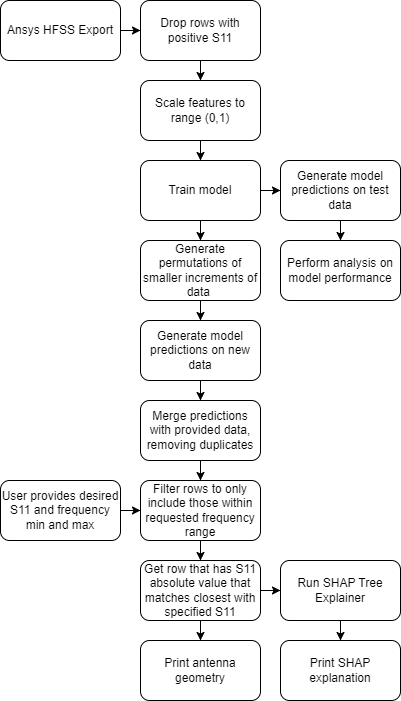
\includegraphics[width=2.25in]{methodology}
\captionof{figure}{Flow of data through the system}
\label{data_flow}
\end{Figure}

A GUI (graphical user interface) was created in order to make the process of filtering optimal geometries more intuitive. The GUI include an input area, where a user can input a desired $S_{11}$ and frequency range. Once these are entered, all of the combinations are filtered and the best performing optimal geometries are shown. A graph of frequency and predicted $S_{11}$ is also shown, where each optimal geometry is plotted. The desired $S_{11}$ and frequency range are also represented on the graph so it's clear what area of the graph is being focused on.


\section{Results}
\subsection{Library and Model Comparison with the Patch Antenna}
All of the Scikit-learn regression models had decent accuracies. After performing a randomized search for the best hyperparameters for each model, the score of the best configuration of each model was reported with the $R^2$ and RMSE scores in Table~\ref{comparing_sklearn}. The table is sorted by best to worst performance by score, RMSE, and $R^2$. The goal is to have the accuracy and $R^2$ closest to one, and the RMSE closest to zero. 

It's clear by looking at the table that XGBRegressor and RandomForestRegressor are the best performing models. They have the highest accuracy and the lowest RMSE, which proves that its predictions had the least distance from the actual $S_{11}$ values. The RandomForestRegressor model will ultimately be the model that is used because the decision trees that it is based on are not sensitive to outliers, where XGBRegressor is~\cite{BROWN2009541,Li_2018}. 

\begin{table}[h]
\caption{Scikit-learn Results}
\begin{center}
\begin{tabular}{ |l|l|l|l| }
    \hline
    Model Type & Accuracy within~$\pm$1dB & RMSE & $R^2$ \\ 
    \hline
    XGBRegressor & 0.9410 & 0.7330 & 0.9651 \\  
    \hline
    RandomForestRegressor & 0.9286 & 0.7717 & 0.9614 \\
    \hline  
    GradientBoostingRegressor & 0.9012 & 0.9950 & 0.9357 \\
    \hline
    CatBoostRegressor & 0.8969 & 0.9949 & 0.9358 \\    
    \hline
    DecisionTreeRegressor & 0.8808 & 1.1082 & 0.9202 \\  
    \hline
    AdaBoostRegressor & 0.8523 & 1.1956 & 0.9072 \\  
    \hline
\end{tabular}
\end{center}
\label{comparing_sklearn}
\end{table}

\subsection{Testing with Unseen Geometries}
The chosen model was given a set of six random geometries from the patch antenna that were new to both the training and testing sets. These geometries were part of the combinations that were generated to create the dataset for optimal geometry searching. It's worth noting that each of the geometric parameters that were chosen for the unseen geometries lay within the range of the minimum and maximum value for each respective parameter. Due to the scaling that was performed during the preprocessing steps, any predictions made with geometric parameters that lay outside of the original range of the training data are capped as if the data point outside of the range was actually the corresponding minimum or maximum. 

\begin{Figure}
    \centering
    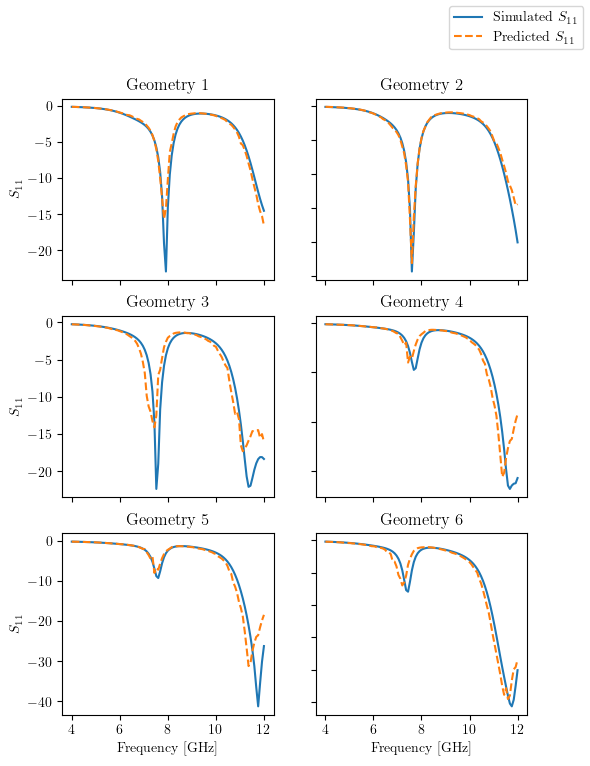
\includegraphics[width=3in]{unseen_geometries_freq_vs_seq}
    \captionof{figure}{Simulated \& Predicted $S_{11}$ Values for Frequency Range of Unseen Geometries}
    \label{unseen_geometries_graph}
\end{Figure}

These unseen geometries were run through both the HFSS and the chosen machine learning model in order to obtain simulated and predicted $S_{11}$ values for the entire frequency range of the patch antenna. The results are shown in Figure~\ref{unseen_geometries_graph}, where each unseen geometry has its simulated $S_{11}$ values plotted alongside the predicted values for each frequency in the frequency range. For all geometries tested, the predicted $S_{11}$ values appear to follow the same trend as the simulated values, but they never reach as far low as the simulated values go. It's interesting to note how the predictions of the $S_{11}$ values of Geometry 2 were nearly identical to the simulated values. For Geometries 3, 4, and 6, both the predicted values and the simulated values had similar dips in the curves around 7GHz and 11GHz. However, the dips were shifted to slightly lower frequency ranges for the predicted values.

\subsection{Finding Optimal Geometry}
A graphical user interface (GUI) was implemented using Jupyter Widgets to allow for ease of exploring different types of geometries~\cite{interactive_Jupyter_widgets}. A user will input a desired $S_{11}$ value and frequency range, and the graph of the predicted $S_{11}$ values for the frequency range wil be output to show the best performing geometries. This graph includes marker lines as a visual aid to show what value the $S_{11}$ predictions should be below and what frequency minimum and maximum the predictions should be between.

An example of an input and the corresponding graph that is generated is shown in Figure~\ref{gui}. The specified $S_{11}$ value of 5dB is represented by the dotted horizontal blue line, and the selected frequency range between 7.47GHz and 8.64GHz is represented by the two dotted vertical green lines. All of the 14 geometries that are found have predicted $S_{11}$ values within these constraints, as represented in the graph. Some geometries create the same exact predictions as one another, so even though all 14 geometries have their predictions plotted, it appears that there are only 3 lines plotted because they are all overlapping one another. Table~\ref{gui_geometries} shows the 14 optimal geometries that are represented in~\ref{gui}. It appears that all geometries that are best for this criteria have a inset\_dist of 0.6mm, L of 11.5mm, and sub\_thick of 2.0mm. The rest of the geometric parameters vary. The biggest advantage of the GUI is the ability to interactively explore which geometric parameters lead to a specified performance and frequency range, where before this was a manual and timely process. 

\begin{Figure}
    \centering
    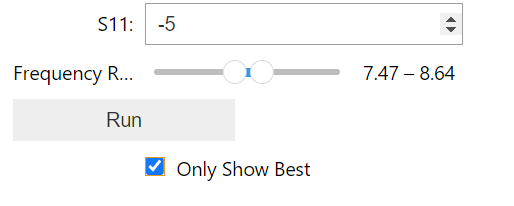
\includegraphics[width=2in]{gui_input}
    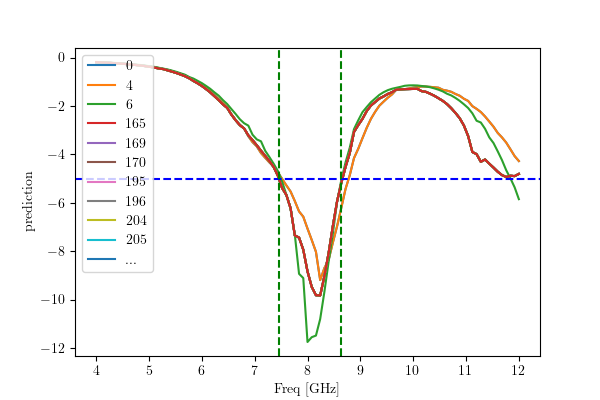
\includegraphics[width=3in]{gui_graph}
    \captionof{figure}{GUI Input and Predicted $S_{11}$ vs Frequency for Optimal Geometries}
    \label{gui}
\end{Figure}

\begin{table}[h]
\caption{Geometries Generated from GUI}
\begin{center}
\begin{tabular}{ |l|p{0.12\linewidth}|l|p{0.12\linewidth}|p{0.07\linewidth}|p{0.07\linewidth}|p{0.07\linewidth}| }
    \hline
    ID & inset\_dist [mm] & L [mm] & sub\_thick [mm] & W [mm] & W0 [mm] & y0 [mm] \\ 
    \hline
    0 & 0.6 & 11.5 & 2.0 & 14.0 & 2.5 & 3.25 \\
    \hline
    4 & 0.6 & 11.5 & 2.0 & 14.0 & 2.75 & 3.0 \\
    \hline
    6 & 0.6 & 11.5 & 2.0 & 14.0 & 2.75 & 3.5 \\
    \hline
    165 & 0.6 & 11.5 & 2.0 & 14.8 & 2.5 & 3.25 \\
    \hline
    169 & 0.6 & 11.5 & 2.0 & 14.8 & 2.75 & 3.0 \\
    \hline
    170 & 0.6 & 11.5 & 2.0 & 14.8 & 2.75 & 3.25 \\
    \hline
    195 & 0.6 & 11.5 & 2.0 & 15.0 & 2.5 & 3.0 \\
    \hline
    196 & 0.6 & 11.5 & 2.0 & 15.0 & 2.5 & 3.25 \\
    \hline
    204 & 0.6 & 11.5 & 2.0 & 15.0 & 2.75 & 3.00 \\
    \hline
    205 & 0.6 & 11.5 & 2.0 & 15.0 & 2.75 & 3.25 \\
    \hline
    240 & 0.6 & 11.5 & 2.0 & 15.2 & 2.5 & 3.00 \\
    \hline
    241 & 0.6 & 11.5 & 2.0 & 15.2 & 2.5 & 3.25 \\
    \hline
    249 & 0.6 & 11.5 & 2.0 & 15.2 & 2.75 & 3.00 \\
    \hline
    250 & 0.6 & 11.5 & 2.0 & 15.2 & 2.75 & 3.25 \\
    \hline
\end{tabular}
\end{center}
\label{gui_geometries}
\end{table}    
    

\section{Conclusion}
Applying a machine learning algorithm as an aid in the process of optimizing antenna geometric parameters with EM simulations greatly reduces the amount of time and computational power required. Training a model on a small set of data obtained from a parameteric sweep allows the model to fit to the trend of data. Large amounts of additional data can then be generated within the bounds of the existing data, and performance predictions can be made for this generated data with a high accuracy. The most optimal geometries can be returned for specified performance values and frequency ranges, making the trial-and-error process of finding these geometries by running simulations unnecessary. 

\bibliographystyle{IEEEtran}
\bibliography{refs}

\vfill

\end{document}